% !tex root = ../Thesis.tex

In this chapter, the results of metrics designed for the frequency detector and
pitch correction system will be given and interpreted. The frequency detector will
be discussed first and the pitch correction system will follow. Some real vocal
recordings will also be corrected using a few different configurations of the
pitch correction system. This is to give some confidence that the system can hadle
real data and doesn't just rely on clean signals the metrics have been designed
for. These examples are not rigorous by nature and should just be considered as a
final real world demonstaration.

\section{Frequency Detector}

The noise robustness metric for each of the two pitch detection algorithms were
run. This checks how much noise can be introduced into a signal with a known pitch
contour before the pitch detector produces unacceptable results. Unacceptable is
seen as having a mean squared pitch error of more than $0.59\times10^-6$. The
metric will be quoted in decibels of noise.

Figure \ref{fig:NoiseRobustnessZCM} shows a graph plotting the square pitch error,
of the Zero Crossing frequency detector, as a function of additive noise in
decibels. The square pitch error is plotted using $log_{10}$ scaling to make the
graph more readable.

\begin{figure}[h]
	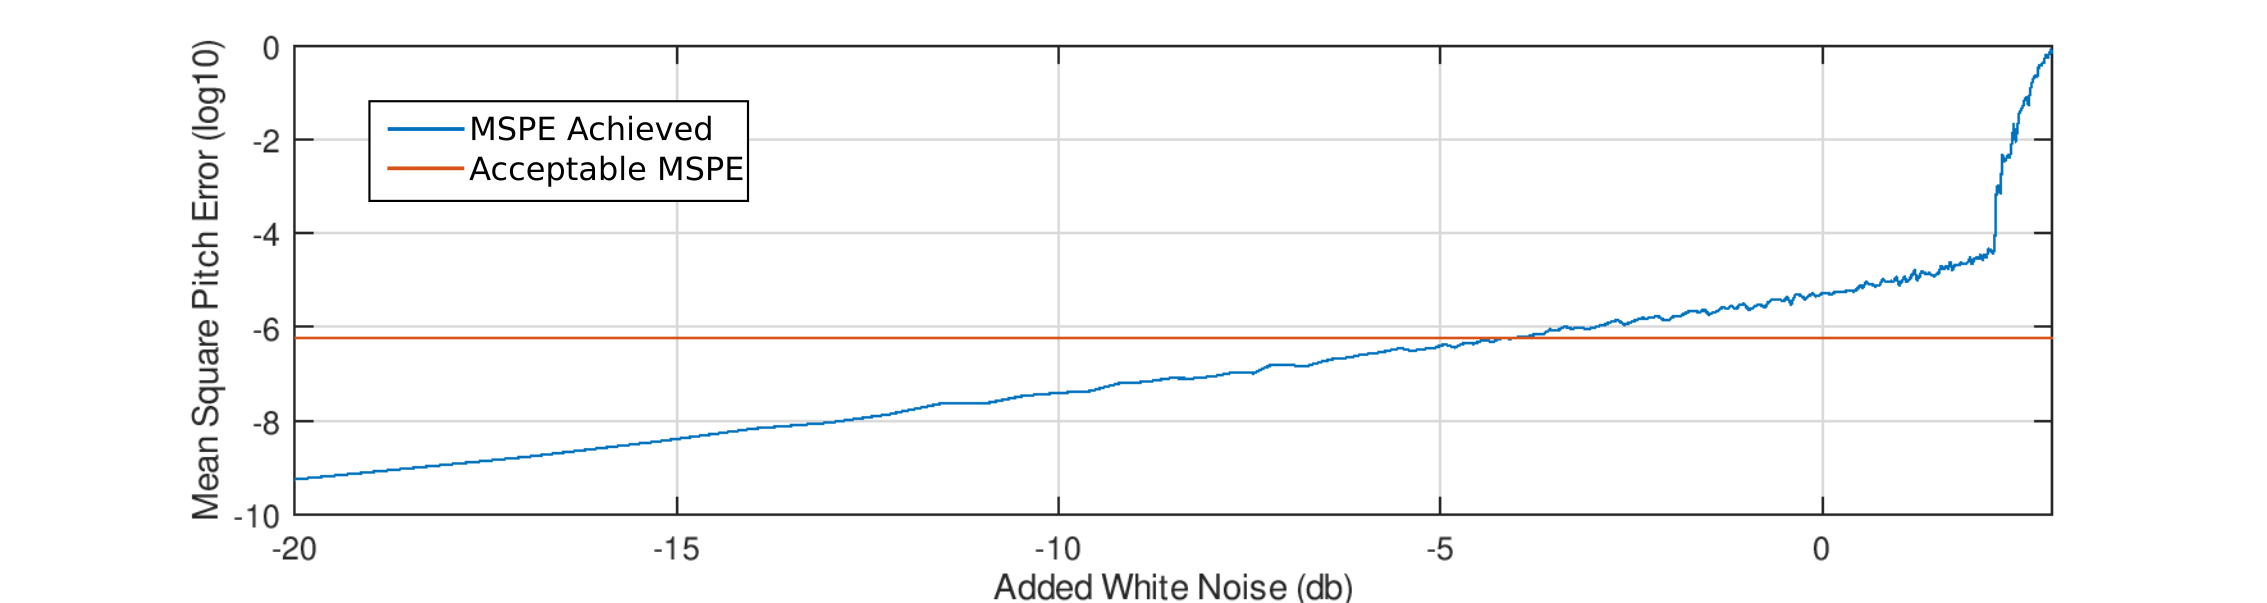
\includegraphics[width=\textwidth,trim={2.5cm 0mm 2.5cm 0mm},clip]
	{NoiseRobustnessZCM}
	\caption{Zero Crossing Method Noise Robustness}
	\label{fig:NoiseRobustnessZCM}
\end{figure}

Since the input signal has an amplitude of 0 decibel, the signal to noise ratio
can easily be determined. The graph shows that the zero crossing method requires a
SNR of 4.5db in order to function at a acceptable level.

Figure \ref{fig:NoiseRobustnessAutoCorr} shows a similar graph but of the
autocorrelation method. The SNR required for acceptable performance is 17.8db.
This is worse than the expected and indicates an error in implementation. It is
postulated that this is a resolution error and oversampling of the signal before
autocorrelation is required. It is also worth mentioning that very little time was
spent inspecting the autocorrelation code and that mistakes are highly likely.

\begin{figure}[h]
	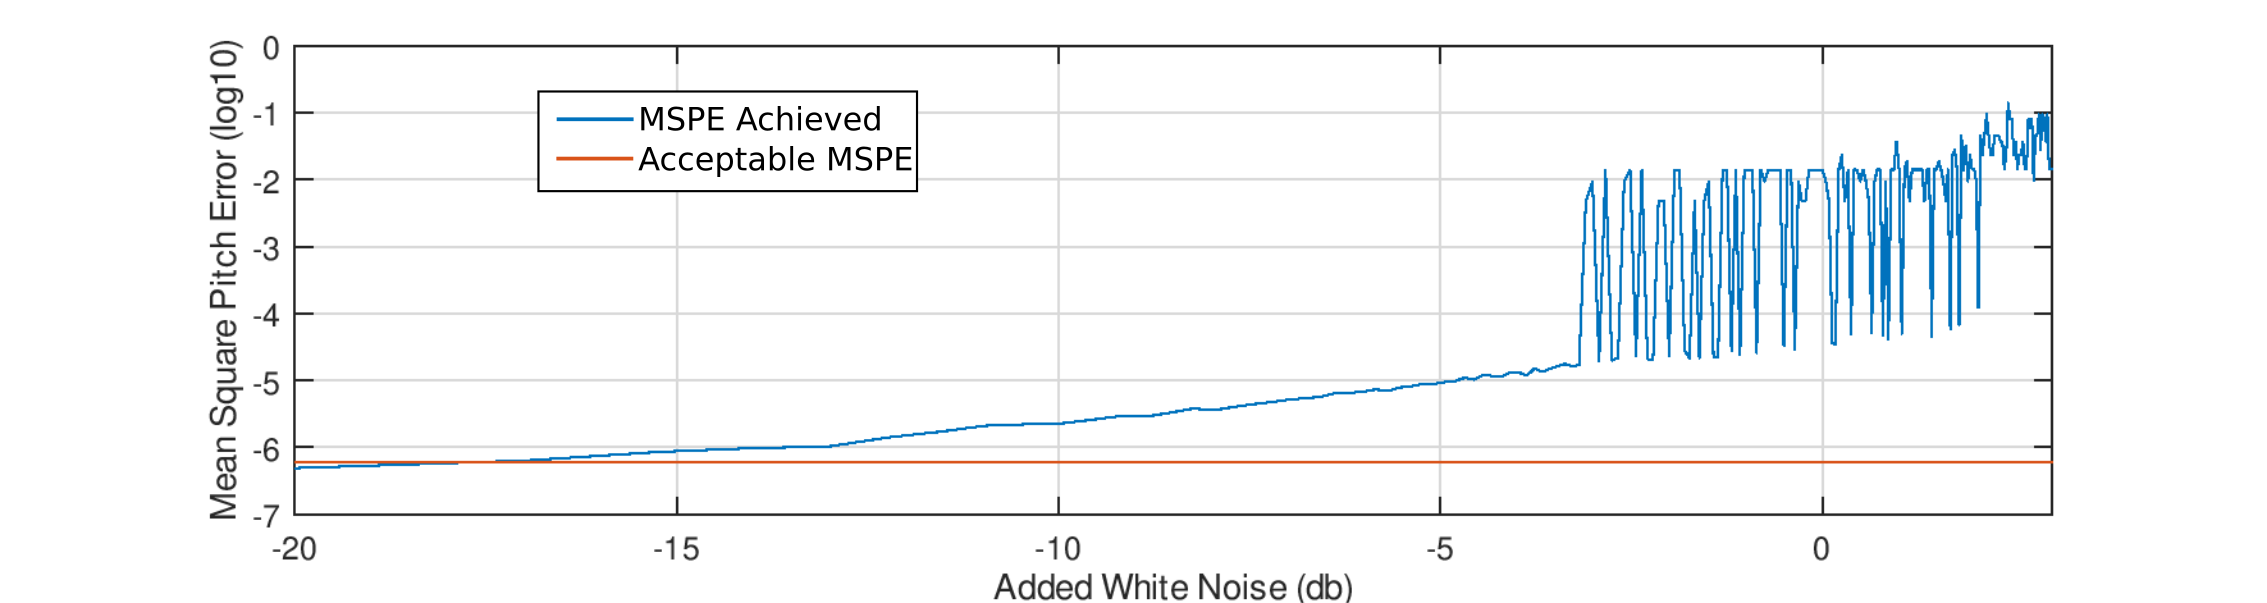
\includegraphics[width=\textwidth,trim={2.5cm 0mm 2.5cm 0mm},clip]
	{NoiseRobustnessAutoCorr}
	\caption{Autocorrelation Method Noise Robustness}
	\label{fig:NoiseRobustnessAutoCorr}
\end{figure}

\section{Pitch Corrector}

Because of time constraints, only the combination of the zero-crossing method and
the phase vocoder, as sub-modules, will be tested. This combination does also seem
like the most likely combination to produce the best results. This is because of
the results seen when testing the sub-modules individually and during the
development of the modules.

The first metric to test is the effectiveness metric. The goal is to produce a
number to say: ``The pitch corrector improves the pitch accuracy by X times''.
Figure \ref{fig:EffectivenessPVZCM} shows the pitch contour plot of the test
defined in the implementation chapter.

\begin{figure}[h]
	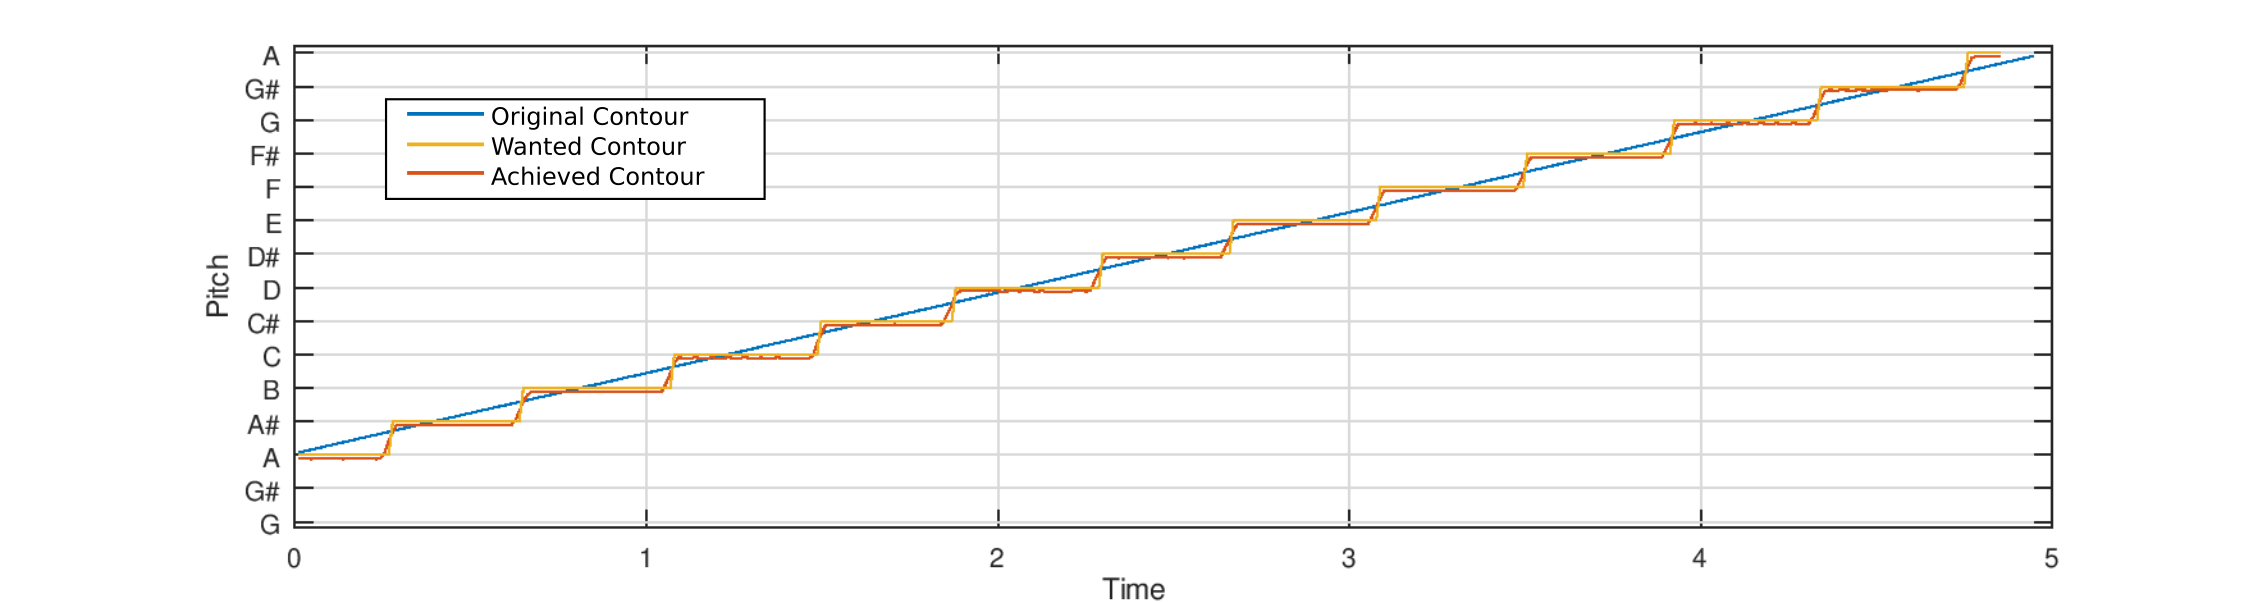
\includegraphics[width=\textwidth,trim={2.7cm 0mm 2.7cm 0mm},clip]
	{EffectivenessPVZCM}
	\caption{Autocorrelation Method Noise Robustness}
	\label{fig:EffectivenessPVZCM}
\end{figure}

The achieved pitch contour very narrowly follows the wanted pitch contour. The
mean squared pitch error before the correction was $0.59 \times 10^{-3}$, and
after the correction, $0.13 \times 10^{-3}$. This results in a pitch accuracy
improvement factor of 4.38.

\color{red}
To do:
\begin{itemize}
	\item Include distortion metric
\end{itemize}
\color{black}
